\documentclass[
	% -- opções da classe memoir --
	12pt,				% tamanho da fonte
	openright,			% capítulos começam em pág ímpar (insere página vazia caso preciso)
	oneside,			% para impressão em verso e anverso. Oposto a oneside
	a4paper,			% tamanho do papel.
	% -- opções da classe abntex2 --
	% chapter=TITLE,                  % títulos de capítulos convertidos em letras maiúsculas
	% section=TITLE,		  % títulos de seções convertidos em letras maiúsculas
	% subsection=TITLE,               % títulos de subseções convertidos em letras maiúsculas
	% subsubsection=TITLE,            % títulos de subsubseções convertidos em letras maiúsculas
	% -- opções do pacote babel --
	english,			% idioma adicional para hifenização
	french,				% idioma adicional para hifenização
	spanish,			% idioma adicional para hifenização
	brazil				% o último idioma é o principal do documento
	]{abntex2}

% ---
% Pacotes básicos
% ---
\usepackage{lmodern}			% Usa a fonte Latin Modern
\usepackage[T1]{fontenc}		% Selecao de codigos de fonte.
\usepackage[utf8]{inputenc}		% Codificacao do documento (conversão automática dos acentos)
\usepackage{lastpage}			% Usado pela Ficha catalográfica
\usepackage{indentfirst}		% Indenta o primeiro parágrafo de cada seção.
\usepackage[usenames,dvipsnames]{color} % Controle das cores
\usepackage{graphicx}			% Inclusão de gráficos
\usepackage{microtype} 			% para melhorias de justificação
\usepackage[chapter]{algorithm}
\usepackage[noend]{algorithmic}
\usepackage{graphicx,url}  % for using figures and url format
\usepackage{wrapfig}
\usepackage{algorithm}
\usepackage[noend]{algorithmic}
\usepackage{amsmath}
\usepackage{mathtools}
\usepackage[normalem]{ulem}
% ---

\addto\captionsbrazil{
%% ajusta nomes padroes do babel
\renewcommand{\bibname}{REFER\^ENCIAS}
\renewcommand{\chaptername}{Seção}
}

% ---
% Pacotes adicionais, usados apenas no âmbito do Modelo Canônico do abnteX2
% ---
\usepackage{lipsum}                          % para geração de dummy text
% ---

% ---
% Pacotes de citações
% ---
\usepackage[brazilian,hyperpageref]{backref} % Paginas com as citações na bibl
\usepackage[alf]{abntex2cite}                % Citações padrão ABNT

% Configurações de fontes
\chapterstyle{abnt}

% ---
% CONFIGURAÇÕES DE FONTES
% ---
\renewcommand{\ABNTEXchapterfont}{\fontfamily{\rmdefault}\fontseries{b}\selectfont}
\renewcommand{\ABNTEXchapterfontsize}{\HUGE}
\renewcommand{\ABNTEXsectionfontsize}{\LARGE}
\renewcommand{\ABNTEXsubsectionfontsize}{\Large}
\renewcommand{\ABNTEXsubsubsectionfontsize}{\large}
\renewcommand{\ABNTEXsubsubsubsectionfontsize}{\large}
\renewcommand{\ABNTEXpartfontsize}{\large}

% ---
% CONFIGURAÇÕES DE PACOTES
% ---

% ---
% Configurações do pacote backref
% Usado sem a opção hyperpageref de backref
\renewcommand{\backrefpagesname}{Citado na(s) página(s):~}
% Texto padrão antes do número das páginas
\renewcommand{\backref}{}
% Define os textos da citação
\renewcommand*{\backrefalt}[4]{
	\ifcase #1 %
		Nenhuma citação no texto.%
	\or
		Citado na página #2.%
	\else
		Citado #1 vezes nas páginas #2.%
	\fi}%
% ---

% ---
% Configurações gráficas
% ---
\DeclareGraphicsExtensions{.png,.eps,.pdf,.jpg} % Preferência por .eps (maior resolução)
\graphicspath{{fig/}}                           % Pasta padrão para as figuras
\usepackage{chngcntr}

\newcommand{\grifar}[1]{\textcolor{Red}{\textbf{#1}}}

\newcommand{\lucas}{Lucas dos Santos Fernandez}
\newcommand{\malu}{Maria Luiza Mondelli}
\newcommand{\rafael}{Rafael Lemes Beirigo}
\newcommand{\tainara}{Tainara Mendes}

% ---
% Informações de dados para CAPA e FOLHA DE ROSTO
% ---
\newcommand{\aut}{\lucas{}, \malu{}, \rafael{}, \tainara{}}
\newcommand{\tit}{Fluxo da Informação em Redes Sociais}
\newcommand{\tipotrab}{Trabalho Final de Disciplina}

\titulo{\tit}
\autor{LABORATÓRIO NACIONAL DE COMPUTAÇÃO CIENTÍFICA}
\local{LNCC}
\data{2015}
\instituicao{%
  \par \textbf{Programa de Pós-Graduação em Modelagem}
  \par \textbf{Disciplina de Fundamentos de Modelagem}
}
\tipotrabalho{\tipotrab}
% O preambulo deve conter o tipo do trabalho, o objetivo,
% o nome da instituição e a área de concentração
\preambulo{\textbf{Alunos:} \newline
  \lucas \newline
  \malu \newline
  \rafael \newline
  \tainara
}
% ---

% ---
% Configurações de aparência do PDF final

% alterando o aspecto da cor azul (utilizado nos links)
\definecolor{blue}{RGB}{0,0,128}

% informações do PDF
\makeatletter
\hypersetup{
    % pagebackref=true,
    pdftitle={\tit},
    pdfauthor={\aut},
    pdfsubject={\imprimirpreambulo},
    pdfcreator={LaTeX with abnTeX2},
    colorlinks=true,       		% false: boxed links; true: colored links
    linkcolor=blue,                     % color of internal links
    citecolor=blue,        		% color of links to bibliography
    filecolor=magenta,      		% color of file links
    urlcolor=blue,
    bookmarksdepth=4
}
\makeatother
% ---

% ---
% Espaçamentos entre linhas e parágrafos
% ---

% O tamanho do parágrafo é dado por:
\setlength{\parindent}{1.3cm}

% Controle do espaçamento entre um parágrafo e outro:
\setlength{\parskip}{0.2cm}  % tente também \onelineskip

% ---
% compila o indice
% ---
\makeindex
% ---

% ----
% Início do documento
% ----
\begin{document}

% Retira espaço extra obsoleto entre as frases.
\frenchspacing

% ----------------------------------------------------------
% ELEMENTOS PRÉ-TEXTUAIS
% ----------------------------------------------------------
\pretextual

\imprimirfolhaderosto

% ---
% inserir o sumario
% ---
\pdfbookmark[0]{\contentsname}{toc}
\tableofcontents*
\cleardoublepage
% ---

% ----------------------------------------------------------
% ELEMENTOS TEXTUAIS
% ----------------------------------------------------------
\textual

\chapter[Introdução]{Introdução}
Há cerca de um ano, dois meninos do interior do Vale do Itajaí, Santa
Catarina, gravavam um vídeo de uma de suas brincadeiras. Numa rua de
chão de terra, num ponto mais alto, vinha o mais velho dos dois em
cima de um carrinho de rolimã tentando obter mais e mais velocidade
naquela corrida sem competidores, enquanto o mais jovem narrava a
descida do primo sobre o carrinho. Uma brincadeira simples, do dia a
dia de duas crianças, e que tinha tudo para permanecer ali, na
história deles dois, não fosse a ideia de um deles de postar o vídeo
no Youtube. O vídeo foi um sucesso, mas não imediato. Alguns meses
foram necessários, até que alguém, não se sabe onde e não se sabe o
porquê, assistiu o vídeo e compartilhou com os amigos de um grupo do
Whatsapp. De compartilhamento em compartilhamento, o vídeo virou um
sucesso e alcançou mais grupos do Whatsapp, depois Facebook e
Twitter. O vídeo original conta hoje com mais de seis milhões de
visualizações. Por algum motivo, esse simples vídeo que mostra um
breve momento na vida de duas crianças foi capaz de gerar uma onda de
comportamentos sociais a partir da temática ali existente. Emissoras
de televisão fizeram gravações com os meninos, corridas com carrinhos
de rolimã começaram a ressurgir em inúmeros municípios, principalmente
da região Sul do Brasil, e hoje, já há algum tempo daquele momento
ápice de fama dos dois meninos, é provável que alguém esteja
assistindo ao vídeo e comentando com amigos ou compartilhando em seus
perfis nas redes sociais.

O relato acima é apenas um exemplo dos muito existentes deste mesmo
tipo. A Internet e as redes sociais são hoje um mecanismo de
comunicação intensa, de constante troca de conhecimento e de visível
influência sob a vida humana e, acredite, essa influência não é sutil
nem mesmo involuntária. Pelo contrário, neste momento, profissionais
da ciência da computação estão buscando implementar códigos mais
eficientes para que você encontre um tópico mais rapidamente, para que
uma propaganda de impacto e do seu interesse apareça na sua tela, para
que você esteja conectado aos seus amigos mais próximos e possa então
ter conhecimento sobre os textos, vídeos, artigos de jornal, gifs,
memes e outras tantas entidades do mundo virtual que eles venham a
postar na Internet, seja nos seus perfis nas redes sociais, blogs ou
sites.

Quando você digita uma única palavra na busca do Google, dependendo da
palavra, o site imediatamente lista composições de palavras que
provavelmente condiz com aquilo que você quer pesquisar. Se você curte
muitos perfis ou páginas de esportes no Facebook, por exemplo, então
provavelmente haverá mais propaganda de esportes na sua página dessa
rede social. Se você, num círculo de amigos em uma rede social, possui
mais influência que os demais, então é provável que uma postagem sua
tenha mais impacto e se espalhe mais rapidamente no meio virtual que
qualquer outra postagem de qualquer um dos seus amigos.

Todos os fenômenos mencionados no parágrafo anterior podem ser
perfeitamente explicados por meio de códigos computacionais, da
ciência existente por trás dos computadores e da dinâmica do mundo
virtual. Cada usuário da Internet, principalmente e certamente nas
redes sociais, está conectado a outros inúmeros usuários de modo que
cada um destes usuários determina uma rede que faz parte de uma rede
maior, incrivelmente grande, já que a Internet está presente num
considerável número de países. A informação é o objeto de todo usuário
virtual.

As informações, de natureza e relevância as mais variadas, estão, a
cada segundo, sendo lançadas por esses usuários no meio virtual. Mais
diretamente, é preciso frisar que a informação é o alimento da
Internet e das redes sociais, ou seja, é a informação que mantém a
Internet ativa e renovada. Consequentemente, é a informação que mantém
os usuários online, hora após hora, dia após dia, e é a busca por
informação e também a curiosidade que fazem com que usuários deixem a
Internet por algumas horas e logo em seguida voltem para obter mais
informações.

O fluxo de informações na Internet é um processo dinâmico e curioso. O
modo como as redes sociais se utilizam de nossas preferências para
sugerir a compra de um produto ou de um serviço e o espalhamento de
uma postagem são só alguns exemplos de como as redes virtuais atuam no
nosso dia a dia. Esse fluxo de informações mostra ao usuário ativo da
Internet tanto o uso responsável das informações quanto o uso
irresponsável e, muitas vezes, até desnecessário. Em outras palavras,
há nas redes sociais uma mistura de informações verídicas, de rumores
(os boatos) e de informações falsas que podem ser veiculadas por um
longo período de tempo, dependendo das redes de usuários e do
interesse desses usuários nas informações que ali são veiculadas.

Nesse contexto, dentre inúmeras indagações, perguntamo-nos: "o que
determina o espalhamento de uma informação?", "quanto tempo uma
notícia com alto potencial de repercussão permanece veiculada no meio
virtual?", "o potencial de uma informação está diretamente relacionada
à rede de usuários determinada pelo usuário que lançou a informação no
meio virtual?", "se um usuário é influente, qual o impacto de uma
informação veiculada por este usuário?", "como modelar a interação
entre os usuários e as informações?". Estes questionamentos motivam e
justificam a modelagem que se objetiva investigar neste trabalho.

Dadas as complexidades envolvidas na análise e matematização da
interação entre usuários em uma rede social, este trabalho terá como
objetivo modelar a taxa de propagação de uma informação em uma rede
social. Para isto, serão apresentados os modelos físico e matemático
do fenômeno e, em seguida, será proposto um meio de resolução do
modelo e serão apresentadas críticas a este modelo.


\chapter{Modelo Físico}
A partir das observações e considerações realizadas, será apresentado
o modelo físico e suas variáveis a fim de tornar possível a modelagem
matemática do problema abordado neste trabalho. Utilizaremos como
referência os modelos de transmissão de doenças pelo fato de serem
semelhantes aos modelos que descrevem processos de contágio social,
uma vez que tanto a doença quanto a informação podem ser transmitidas
em uma população e adquiridas por um indivíduo, a partir do momento em
que ele esteja suscetível. Sendo assim, utilizaremos alguns conceitos
epidemiológicos para a descrição do modelo proposto.

Observamos que grafos podem ser utilizados para representar redes de
contato em Epidemiologia. Percebemos que o mesmo tipo de estrutura
pode ser utilizado para representar uma rede social. Por este motivo,
neste trabalho consideramos que os nós são constituídos pelos usuários
da rede, o contato direto da informação entre esses usuários é
representado pelas linhas cheias e o contato indireto da informação
com esses usuários pelas linhas pontilhadas, conforme representado
pela Figura~\ref{fig:grafo}.

\begin{center}
    \begin{figure}
      \begin{center}
        \setlength\fboxsep{0pt}
        \setlength\fboxrule{0pt}
        \fbox{\includegraphics[width=0.6\textwidth]{grafo}}
        \caption{Representação de uma rede social em forma de grafo}
        \label{fig:grafo}
      \end{center}
    \end{figure}
\end{center}

Consideramos uma rede social que permita a propagação de uma
determinada informação que se quer veicular. Considere que a rede
social possui $N$ usuários cadastrados, aptos a receber e transmitir
informação. Deste modo, $N$ representa a população total que
possibilitará a transmissão da informação.

Neste trabalho utilizamos o modelo epidemiológico
SIR~\cite{hethcote2000}, fazendo uma analogia entre a transmissão de
uma doença e o compartilhamento de uma informação.  Assim, conforme
determinada informação passa a ser veiculada na rede social, estes $N$
usuários passam a ser divididos por grupos, a saber, o grupo dos
usuários suscetíveis ($S$) que são aqueles que tiveram contato direto
ou indireto com a informação, dos infectados ($I$) que são aqueles que
receberam e acessaram a informação e podem ou não compartilhá-la; e
dos recuperados ($R$) que são aqueles que foram infectados e podem ou
não acessar novamente a mesma informação. Cada um destes grupos é
dividido em outros dois nomeados receptivos e resistentes. Deste modo,
tem-se os seguintes grupos e suas descrições:

\begin{itemize}
\item $S_1$: suscetível-receptivo - usuário que teve contato direto com a informação;
\item $S_2$: suscetível-resistente - usuário que teve contato indireto com a informação;
\item $I_1$: infectado-receptivo - usuário que teve contato, acessou e compartilhou a informação;
\item $I_2$: infectado-resistente - usuário que teve contato, acessou e não compartilhou a informação;
\item $R_1$: recuperado-receptivo - usuário que foi infectado e que pode acessar novamente a informação
\item $R_2$: recuperado-resistente - usuário que foi infectado e que não quer acessar novamente a informação
\end{itemize}

A transmissão da informação entre os usuários neste modelo ocorre
através do contato direto entre os suscetíveis e infectados de acordo
com a Lei de Ação das Massas (LAME) em epidemiologia, que tem sua
origem no estudo da cinética química. Também conhecida como princípio
de ação das massas, essa lei postula que a taxa de formação de um
composto é proporcional às concentrações dos reagentes. Esta suposição
justifica-se em níveis de concentração suficientemente baixos, para
que cada molécula possa se movimentar independentemente das
demais. Desta forma, ao aumentar-se a concentração de reagentes,
aumenta-se proporcionalmente o número de colisões entre as moléculas
que levam à formação do composto final~\cite{coutinho2004}.

\begin{center}
    \begin{figure}
      \begin{center}
        \setlength\fboxsep{0pt}
        \setlength\fboxrule{0pt}
        \fbox{\includegraphics[width=0.9\textwidth]{diagramadefluxo}}
        \caption{Diagrama de fluxo do modelo de transmissão de
          informação. As setas pontilhadas indicam apenas o contato
          entre os usuários suscetíveis e infectados}
        \label{fig:diagramadefluxo}
      \end{center}
    \end{figure}
\end{center}

O princípio de ação das massas é traduzido para a epidemiologia por
meio da ideia de que a disseminação da epidemia em uma população é
proporcional ao produto da densidade de indivíduos suscetíveis pela
densidade de indivíduos infecciosos~\cite{massad1996}. Este princípio
foi originalmente formulado por meio de um modelo de tempo discreto e
supõe que os indivíduos infecciosos misturam-se homogeneamente aos
suscetíveis em toda a população. Porém, a pesquisa epidemiológica já
mostrou que as heterogeneidades intervêm no processo de transmissão
~\cite{coutinho2004}. Sendo assim, a consideração acima não é
verdadeira.

É importante ressaltar que, de forma diferente ao que ocorre na
maioria dos modelos epidemiológicos, aqui não faremos distinção entre
indivíduos infecciosos e infectados, ou seja, no momento em que o
usuário da rede acessa a informação ele torna-se ``infectado'' e,
portanto, transmissor da informação. Além disso, esses agentes
transmissores da informação mantêm suas características, ou seja, o
grupo $I_1$ representa o conjunto dos usuários que são mais
receptíveis à informação e também possuem maior capacidade de
compartilhamento desta. No grupo $I_2$ estão os usuários com menor
capacidade ou interesse em difundi-las e assim não compartilham a
informação~\cite{pachi2006}.

Conforme o modelo SIR, as variáveis $N$, $S_1$, $S_2$, $I_1$, $I_2$,
$R_1$ e $R_2$ representam a quantidade de indivíduos no tempo $t$,
medido em segundos.


\chapter{Modelo Matemático}
A partir do modelo físico descrito na seção anterior será desenvolvida
aqui uma formulação matemática que represente o fluxo de informação em
redes sociais. O objetivo deste trabalho é, portanto, determinar a
taxa de propagação de uma informação em uma rede social, considerando
o esquema de divisão da população descrita no modelo físico.

Considerando que a transmissão de informação ocorre segundo a LAME, a
probabilidade de encontro entre um usuário suscetível e um infectado é
proporcional ao número de usuários infecciosos da população na qual a
informação está sendo divulgada, ou seja, $\beta SI / N$. Em nosso
estudo, $\beta$ é o coeficiente de transmissão da informação e
representa a taxa de contato entre esses usuários suscetíveis e
infectados por unidade de tempo.

Desta forma, o contato entre os usuários $S_i$ e $I_i$ ocorre a uma
taxa $\beta_i$, onde $i \in \{1,2\}$. Porém, os usuários infectados
$I_2$ influenciam os usuários $S_1$, mais receptíveis à informação, a
uma taxa $\beta_3 = \sigma \beta_1$, e também influenciam os usuários
$S_2$, menos receptíveis à informação, a uma taxa $\beta_4 = \sigma
\beta_2$. O parâmetro $\sigma$ representa a eficiência dos usuários
$I_2$ na transmissão da informação de modo que se $\sigma = 0$ a
transmissão não ocorre e se $\sigma = 1$ a transmissão é perfeita. Num
contexto realista de uma rede social, uma informação é acessada por
alguns usuários, mas não por todos eles. Sendo assim, assumimos $0 <
\sigma < 1$.

Consideramos também a situação na qual uma vez infectados pela
informação acessada, os usuários infectados recuperam-se depois de
certo período de tempo, esquecendo-se da informação e passando a fazer
parte do grupo dos recuperados, $R_1$ e $R_2$, a uma taxa de
esquecimento $\gamma_1$ e $\gamma_2$, respectivamente. Assim,
$\gamma_1^{-1}$ e $\gamma_2^{-1}$ representam os tempos nos quais os usuários
permanecem contaminados pela informação. Sob o aspecto epidemiológico,
tal situação representa a ação do sistema imunológico sobre os
indivíduos infectados que recuperam-se da doença.

No modelo proposto, $\mu$ representa a taxa segundo a qual os usuários
deixam a rede, desativando ou excluindo suas contas. Também existe um
fluxo de entrada $\pi$ de novos usuários que ingressam na rede ao
criarem suas contas. Esse novos usuários ingressam na condição de
suscetíveis segundo determinada proporção $p$. Assim, $p\pi$ ingressam
em $S_1$ e $(1-p)\pi$ ingressam em $S_2$, onde $0 < p < 1$.

Note que, como o fenômeno de interesse monitora o fluxo de uma
informação a partir dos usuários em uma rede social, assume-se que
todos os parâmetros e variáveis do modelo são não negativos.

Dessa forma, com base nos modelos epidemiológicos já existentes na
literatura e nas observações feitas anteriormente, propomos o seguinte
modelo para a propagação de informação em uma rede social:

\begin{equation*}
  \left\{ \begin{aligned}
  \frac{dS_1}{dt} &= (1-p)\pi N - \frac{\beta_1 S_1 I_1}{N} - \frac{\beta_3 S_1 I_2}{N} - \mu S_1 \nonumber \\
  \frac{dS_2}{dt} &= p\pi N - \frac{\beta_4 S_2 I_2}{N} - \frac{\beta_2 S_2 I_1}{N} - \mu S_2 \nonumber \\
  \frac{dI_1}{dt} &= \frac{\beta_1 S_1 I_1}{N} + \frac{\beta_3 S_1 I_2}{N} - (\gamma_1 + \mu)I_1 \nonumber \\
  \frac{dI_2}{dt} &= \frac{\beta_4 S_2 I_2}{N} + \frac{\beta_2 S_2 I_1}{N} - (\gamma_2 + \mu)I_2 \nonumber \\
  \frac{dR_1}{dt} &= \gamma_1 I_1 - \mu R_1 \nonumber \\
  \frac{dR_2}{dt} &= \gamma_2 I_2 - \mu R_2 \nonumber
  \end{aligned}
  \right.
\end{equation*}

%% \grifar{Alternativa com agrupamento por chave (reduz as fontes das frações ):}
%% \begin{align}
%%   \left\{
%%   \begin{array}{lll}
%%   \frac{dS_1}{dt} & = & (1-p)\pi N - \frac{\beta_1 S_1 I_1}{N} - \frac{\beta_3 S_1 I_2}{N} - \mu S_1 \\
%%   \frac{dS_2}{dt} & = & p\pi N - \frac{\beta_4 S_2 I_2}{N} - \frac{\beta_2 S_2 I_1}{N} - \mu S_2 \\
%%   \frac{dI_1}{dt} & = & \frac{\beta_1 S_1 I_1}{N} + \frac{\beta_3 S_1 I_2}{N} - (\gamma_1 + \mu)I_1 \\
%%   \frac{dI_2}{dt} & = & \frac{\beta_4 S_2 I_2}{N} + \frac{\beta_2 S_2 I_1}{N} - (\gamma_2 + \mu)I_2 \\
%%   \frac{dR_1}{dt} & = & \gamma_1 I_1 - \mu R_1 \\
%%   \frac{dR_2}{dt} & = & \gamma_2 I_2 - \mu R_2
%%   \end{array} \nonumber
%%   \right.
%% \end{align}

As condições iniciais para o modelo são:

\begin{equation}
  \begin{array}{ccc}
    S_i(0) = S_i^0 \geq 0, & I_i(0) = I_i^0 \geq 0 & $e$\ R_i(0) = R_i^0 \geq 0,
  \end{array} \nonumber
\end{equation}
\noindent onde $i \in \{1, 2\}$.

Note que

\begin{equation}
  \frac{dN}{dt} = \pi N - \mu N. \nonumber
\end{equation}

Assim, $dN/dt = 0$ se, e somente se, $\pi = \mu$, ou seja, o fluxo de
entrada de novos usuários é igual ao fluxo de saída de usuários da
rede, o que é condizente com o cenário real de uma rede social.


\chapter{Solução do Modelo Matemático}
A epidemiologia matemática é um campo de estudo já estabelecido e com
sólida formalização matemática, geralmente associada a resolução de
equações diferencias ordinárias (EDO) e seus respectivos métodos
numéricos.  A resolução analítica de modelos SIR é possível para
sistemas mais simples, com reduzido número de equações e que
geralmente são utilizados para fins
didáticos~\cite{santos2012}. Contudo, o modelo proposto na seção
anterior trata-se de um sistema de equações diferenciais ordinárias de
primeira ordem não lineares.  Para este tipo de sistema, quanto mais
equações o sistema apresenta, mais complexa e árdua pode se tornar a
sua resolução. Em contraste com a situação para um sistema linear, a
existência e unicidade de solução para um sistema linear não é
garantida~\cite{boyce2003,zill2003}.

Devido ao exposto no parágrafo anterior, para encontrar a trajetória
de um modelo de tempo contínuo, tal como o SIR, integra-se as equações
numericamente, ou seja, aproxima-se as soluções do sistema
computacionalmente.

Diferentes técnicas podem ser empregadas para a resolução de sistemas
de equações diferenciais ordinárias não lineares. Um dos métodos mais
conhecidos e utilizados para a resolução deste tipo de sistema é o
Método de Runge-Kutta multidimensioal. \emph{Softwares} como o
\emph{Python}, \emph{Matlab} e \emph{R} já dispõem de rotinas que
resolvem equações diferenciais ordinárias não lineares e sistemas de
equações deste mesmo tipo. Tais rotinas são chamadas,
\emph{rungek4v.py}, \emph{ode45} e \emph{LSODA}, respectivamente.

Contudo, outros métodos de resolução podem ser encontrados em
trabalhos que tratam da solução numérica do modelo SIR, a saber, o
Método da Transformação Diferencial (MTD) e o Método da Iteração
Variacional (MIV). As principais vantagens do MTD é que ele pode ser
aplicado diretamente a EDO's não lineares sem a exigência de
linearização, discretização ou perturbação, além de ser capaz de
reduzir significativamente o trabalho computacional com alta precisão
nos cálculos, fornecendo a solução da série com taxa de convergência
rápida. Já o MIV, por sua vez, não requer uma transformação específica
para termos não lineares, como acontece para outros métodos numéricos
e a solução é dada em uma série infinita geralmente convergente para a
solução com boa acurácia~\cite{akinboro2014}.


\chapter{Críticas}
Neste trabalho não estamos considerando a existência de mais de um
tipo de conteúdo, ou seja, mais de uma categoria de informação.  Um
anúncio publicitário, uma imagem, um texto e um vídeo são
representações diferentes de informações: diferem no formato, na
linguagem e no estilo, pois buscam transmitir ideias diferentes e
atingir públicos diferentes, mas têm o mesmo propósito, informar algo
a alguém.  Sendo assim, é uma limitação deste modelo não tratar a
diferença entre os diversos tipos de informação.

Ademais, o modelo aqui proposto considera apenas uma rede social,
enquanto na realidade os usuários costumam compartilhar a mesma
informação em diversas redes sociais.  Além disso, existem mecanismos
de interligação entre as redes, o que permite aos usuários
compartilhar a mesma informação em várias redes com facilidade.

Em um cenário real, cada usuário possui determinada influência sobre
outros usuários no momento em que compartilha uma informação.  Dessa
maneira, as informações compartilhadas por este usuário podem chegar a
mais ou menos usuários, propagando-se de forma assimétrica pelas
diferentes regiões do grafo que representa a rede social.  Sendo
assim, é também uma limitação do modelo proposto considerar que a
informação se propaga de forma homogênea no grafo.

Outra característica importante no processo de propagação da
informação em redes sociais, não tratada pelo modelo, é o
\emph{horário} no qual o usuário a compartilha.  Por exemplo, aos
finais de semana, há uma quantidade maior de usuários conectados à
rede, o que também acontece em diferentes períodos do dia ao decorrer
da semana.  Dessa forma, pode-se otimizar a propagação da informação
ao selecionar horários com uma maior quantidade de usuários conectados
à rede.

Apesar de simplificado, o modelo proposto consegue captar
aspectos realísticos, observados em uma rede social, como:

\begin{itemize}
\item nem todo usuário infectado compartilha a informação, podendo o
  usuário acessar a informação, tomando conhecimento dela, mas não
  a compartilhando com outros usuários
\item um usuário recuperado pode se tornar novamente suscetível e
  infectado, o que simula a situação na qual um usuário compartilha a
  mesma informação mais de uma vez em uma rede social, após um período
  de tempo, sendo isto possível no modelo em virtude das taxas de
  esquecimento $\gamma_1$ e $\gamma_2$.
\end{itemize}


% ----------------------------------------------------------
% ELEMENTOS PÓS-TEXTUAIS
% ----------------------------------------------------------
\postextual
% ----------------------------------------------------------

% ----------------------------------------------------------
% Referências bibliográficas
% ----------------------------------------------------------
\citeoption{abnt-etal-list=0}
\bibliography{trabalho}


\end{document}
